%
% $Id: $
%
%
% Compilar a .pdf con LaTeX (pdflatex)
% Es necesario instalar Beamer (paquete latex-beamer en Debian)
%

%
% Gr�ficos:
% Los gr�ficos pueden suministrarse en PNG, JPG, TIF, PDF, MPS
% Los EPS deben convertirse a PDF (usar epstopdf)
%

\documentclass{beamer}
\usetheme{Warsaw}
%\usebackgroundtemplate{
\includegraphics[width=\paperwidth]{format/libresoft-bg.png}}
%\usepackage[spanish]{babel}
\usepackage[latin1]{inputenc}
\usepackage{graphics}
\usepackage{amssymb} % Simbolos matematicos
\usepackage{url}
\usepackage{multirow}
\usepackage{subfigure}


%\definecolor{libresoftgreen}{RGB}{162,190,43}
%\definecolor{libresoftblue}{RGB}{0,98,143}

%\setbeamercolor{titlelike}{bg=libresoftgreen}

%% Metadatos del PDF.
\hypersetup{
  pdftitle={On Computational Thinking as a Universal Skill: A review of the latest research on this ability},
  pdfauthor={Gregorio Robles},
  pdfcreator={Kindergarten and Beyond - Lifelong Learning Research Group (KGB-L3) \\ Universidad Rey Juan Carlos},
  pdfproducer=PDFLaTeX,
  pdfsubject={Computational Thinking Research @ URJC},
}
%%

\begin{document}

\title{On Computational Thinking as a Universal Skill}
\subtitle{A review of the latest research on this ability}
\institute{INTEF, Univ. Rey Juan Carlos, Univ. Nacional de Educaci�n a Distancia \\ (Madrid, Spain)}
\author[Moreno-Le�n et al. // jmorenol@gmail.com]{Jes�s Moreno-Le�n, Gregorio Robles, Marcos Rom�n-Gonz�lez}
\date{EDUCON 2018, Santa Cruz de Tenerife, April 19\textsuperscript{th} 2018}


\AtBeginSection{\frame{\sectionpage}}

\frame{
\maketitle
\begin{center}

\includegraphics[width=1.4cm]{format/intef}
\hspace{0.5cm}

\includegraphics[width=3.2cm]{format/urjc}
\hspace{0.5cm}

\includegraphics[width=1.3cm]{format/uned.jpg}
\hspace{0.5cm}

\includegraphics[width=3cm]{format/emadrid.png}
\end{center}
}


% Si el titulo o el autor se quieren acortar para los pies de p�gina
% se pueden redefinir aqu�:
%\title{Titulo corto}
%\author{Autores abreviado}

%% LICENCIA DE REDISTRIBUCION DE LAS TRANSPAS
\frame{
~
\vspace{3cm}

\begin{flushright}

\includegraphics[width=2.2cm]{figs/by-sa}

{\tiny
(cc) 2018 Jes�s Moreno-Le�n, Gregorio Robles, Marcos Rom�n\\
  Some rights reserved. This work licensed under Creative Commons \\
  Attribution-ShareAlike License. To view a copy of full license, see \\
  http://creativecommons.org/licenses/by-sa/3.0/ or write to \\
  Crea  tive Commons, 559 Nathan Abbott Way, Stanford, \\
  California 94305, USA. \\
\ \\
Some of the figures have been taken from the Internet \\
Source, and author and licence if known, is specified. \\
For those images, \emph{fair use} applies.
}
\end{flushright}
}
%%

%--------------------------------------------------------

\begin{frame}
\frametitle{We still don't know what Computational Thinking is...}

\begin{figure}[htb!]
  \centering
  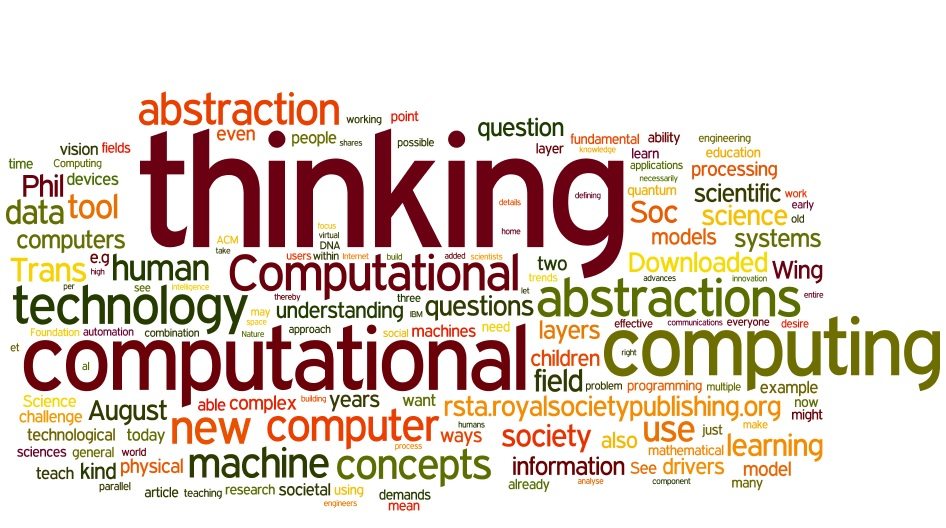
\includegraphics[width=.95\columnwidth]{figs/CT-cloudword.jpg}
  \caption{The term CT is ambiguious and vague}
  \label{fig:CT-cloud}
\end{figure}


\end{frame}

\usebackgroundtemplate{}


%--------------------------------------------------------

\begin{frame}
\frametitle{Great Principles of Computing}

  \begin{columns}[T]
    \begin{column}{0.5\textwidth}
     \begin{block}{The Book}
\begin{figure}[t!]
\begin{center}
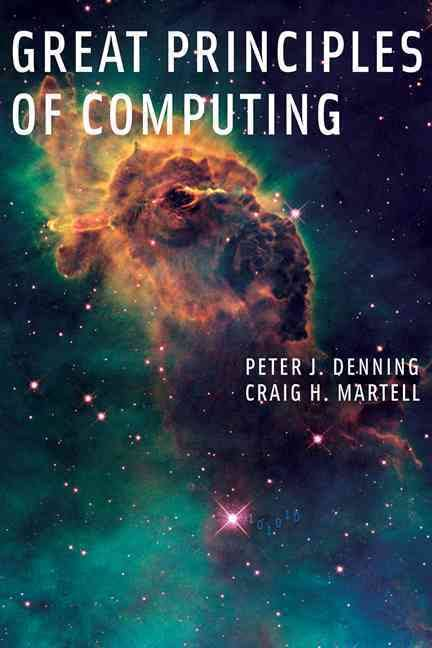
\includegraphics[width=4.4cm,height=5.6cm]{figs/gpc.jpeg}
\end{center}
\label{fig:gpc}
\end{figure}
     \end{block}
    \end{column}
    \begin{column}{0.5\textwidth}
 
     \begin{block}{Seven Principles}
\begin{enumerate}
  \item Information
  \item Machines
  \item Programming
  \item Computation
  \item Memory
  \item Parallelism
  \item Queueing
  \item and Design
\end{enumerate}
     \end{block}

    \end{column}
  \end{columns}


\end{frame}

\usebackgroundtemplate{}



%--------------------------------------------------------

\begin{frame}
\frametitle{Is CT a new skill? (I)}

\begin{figure}[htb!]
  \centering
  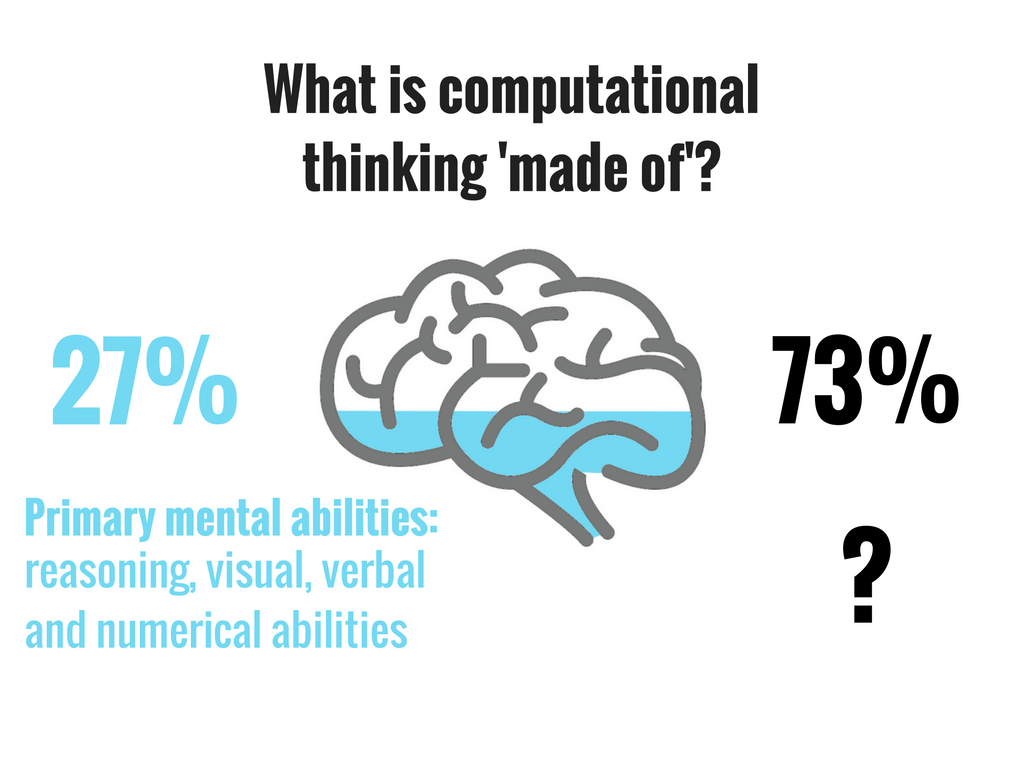
\includegraphics[width=.63\columnwidth]{figs/CT1.png}
  \caption{Computational thinking: only 27\% of its variance can be explained by the four primary mental abilities.}
  \label{fig:CT1}
\end{figure}


\end{frame}

\usebackgroundtemplate{}

%--------------------------------------------------------

\begin{frame}
\frametitle{Is CT a new skill? (and II)}

\begin{figure}[htb!]
  \centering
  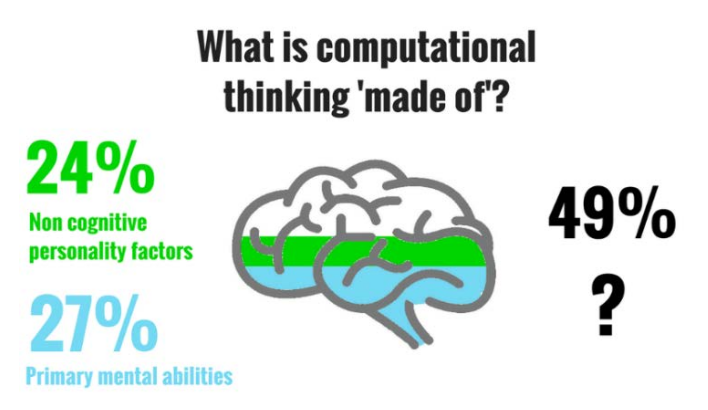
\includegraphics[width=.66\columnwidth]{figs/CT2.png}
  \caption{Computational thinking: only 51\% of its variance can be explained by the four primary mental abilities and non-cognitive personality factors.}
  \label{fig:CT2}
\end{figure}


\end{frame}

\usebackgroundtemplate{}




%--------------------------------------------------------

\begin{frame}
\frametitle{How to develop CT?}


  \begin{columns}[T]
    \begin{column}{0.5\textwidth}
     \begin{block}{Unplugged activities}
\begin{figure}[t!]
\begin{center}
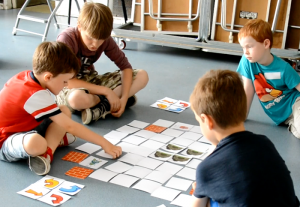
\includegraphics[width=4.4cm,height=3.6cm]{figs/unplugged.png}
\end{center}
\label{fig:unplugged}
\end{figure}
\begin{center}
Unplugged activites \\ (no use of digital devices)
\end{center}
     \end{block}
    \end{column}
    \begin{column}{0.5\textwidth}
 
     \begin{block}{Programming}
\begin{figure}[t!]
\begin{center}
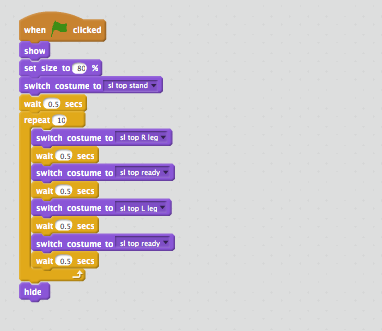
\includegraphics[width=4.4cm,height=4.2cm]{figs/programming.png}
\end{center}
\label{fig:programming}
\end{figure}
\begin{center}
Several ways (arrow-based, block-based, textual, connected to physical world)
\end{center}
     \end{block}
    \end{column}
  \end{columns}


\end{frame}

\usebackgroundtemplate{}

%%--------------------------------------------------------

\begin{frame}
\frametitle{History of learning \emph{with} computers}
\begin{center}
        \begin{figure}[t!]
                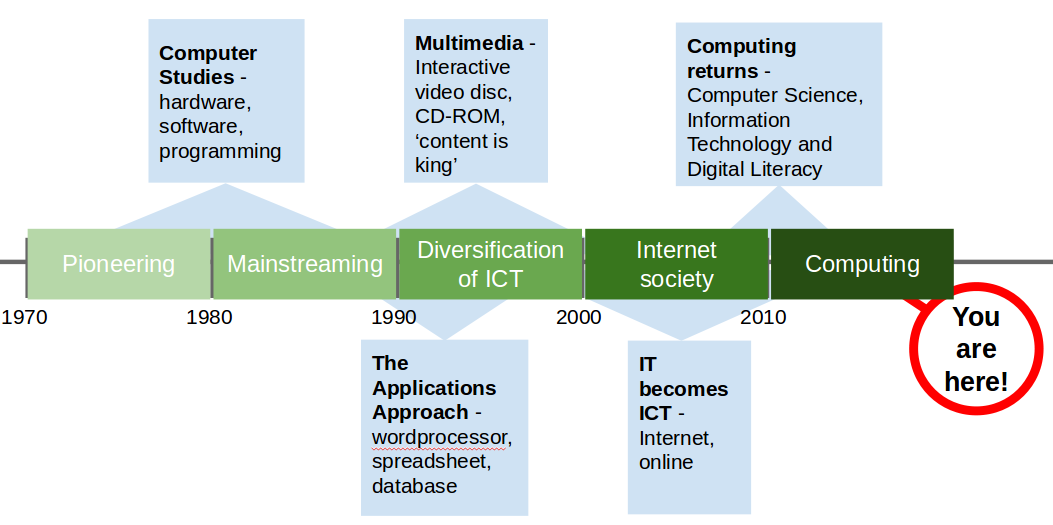
\includegraphics[width=11cm]{figs/history.png}
                \caption{You are here!}
        \end{figure}
        \tiny Source: \textit{REaCT EU project proposal}
\end{center}

\end{frame}

\usebackgroundtemplate{}



%%--------------------------------------------------------

\begin{frame}
\frametitle{Code to learn vs. learn to code}

\vspace{-0.4cm}
\begin{center}
        \begin{figure}[t!]
                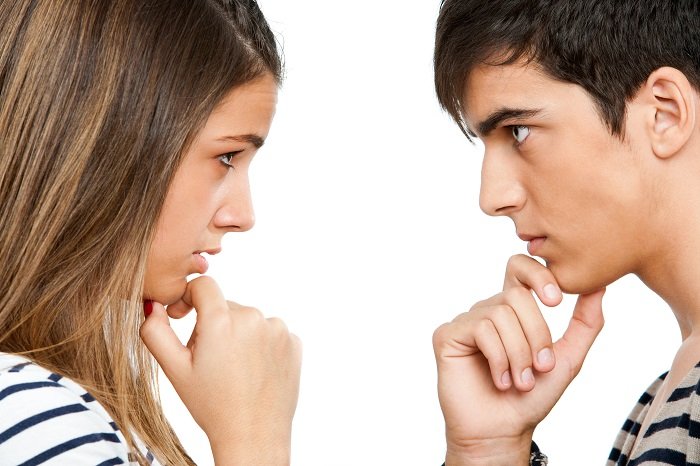
\includegraphics[width=10cm]{figs/facetoface.jpg}
                \caption{Code to learn vs. learn to code}
        \end{figure}
\end{center}

\end{frame}

\usebackgroundtemplate{}


%%--------------------------------------------------------

\usebackgroundtemplate{}
%background: 

\begin{frame}
\frametitle{Maths}

\begin{figure}[h!]
  \centering
	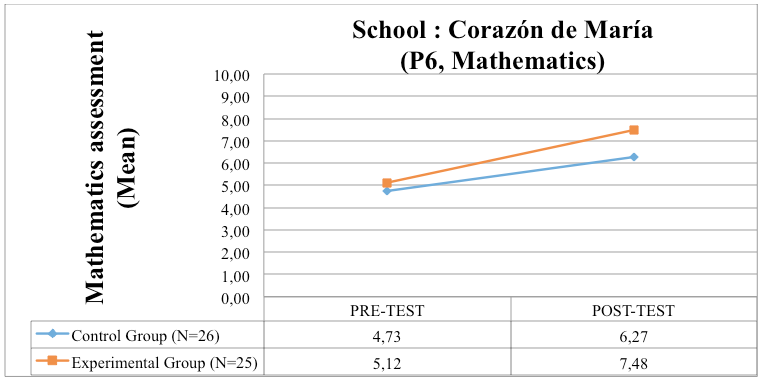
\includegraphics[width=.80\textwidth]{figs/maths.png}
  \caption{Coraz�n de Mar�a school. Comparing the improvement between pre- and post-tests of control and experimental groups.}
  \label{fig:corazon}
\end{figure}

\end{frame}

\usebackgroundtemplate{}


%%--------------------------------------------------------

\usebackgroundtemplate{}
%background: 
    
\begin{frame}
\frametitle{Social sciences}


\begin{figure}[h!]
  \centering
	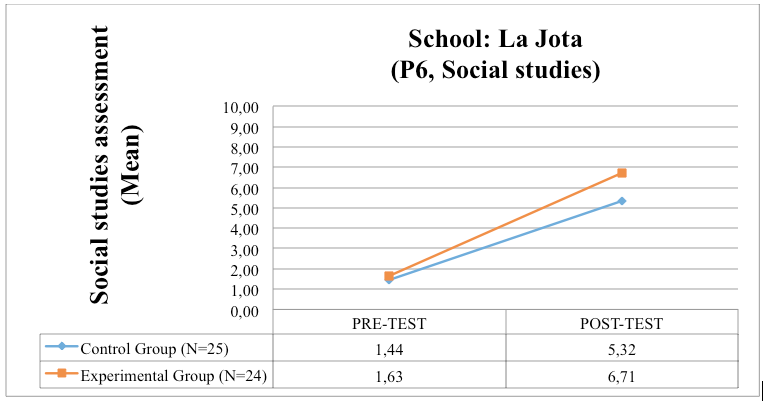
\includegraphics[width=.80\textwidth]{figs/socialstudies.png}
  \caption{La Jota school. Comparing the improvement between pre- and post-tests of control and experimental groups.}
  \label{fig:jota}
\end{figure}

\end{frame}

\usebackgroundtemplate{}

%%--------------------------------------------------------

\usebackgroundtemplate{}
%background: 

\begin{frame}
\frametitle{Arts}


\begin{figure}[h!]
  \centering
	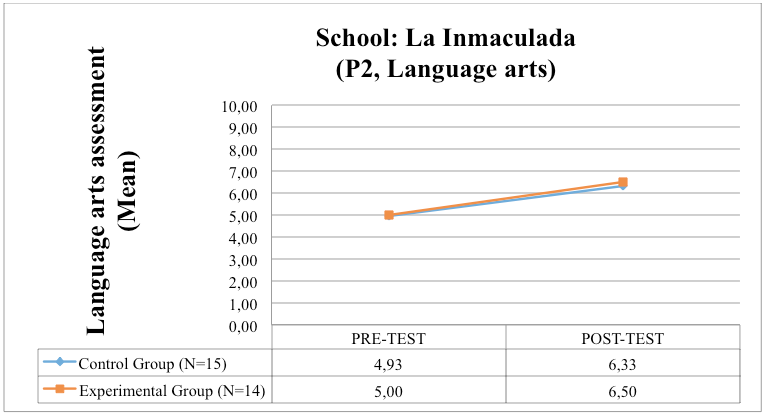
\includegraphics[width=.80\textwidth]{figs/languagearts.png}
  \caption{La Inmaculada school. Comparing the improvement between pre- and post-tests of control and experimental groups.}
  \label{fig:inma}
\end{figure}



\end{frame}

\usebackgroundtemplate{}

%--------------------------------------------------------
\begin{frame}
\frametitle{Social learning}

\begin{figure}[h!]
\begin{subfigure}
  \centering
    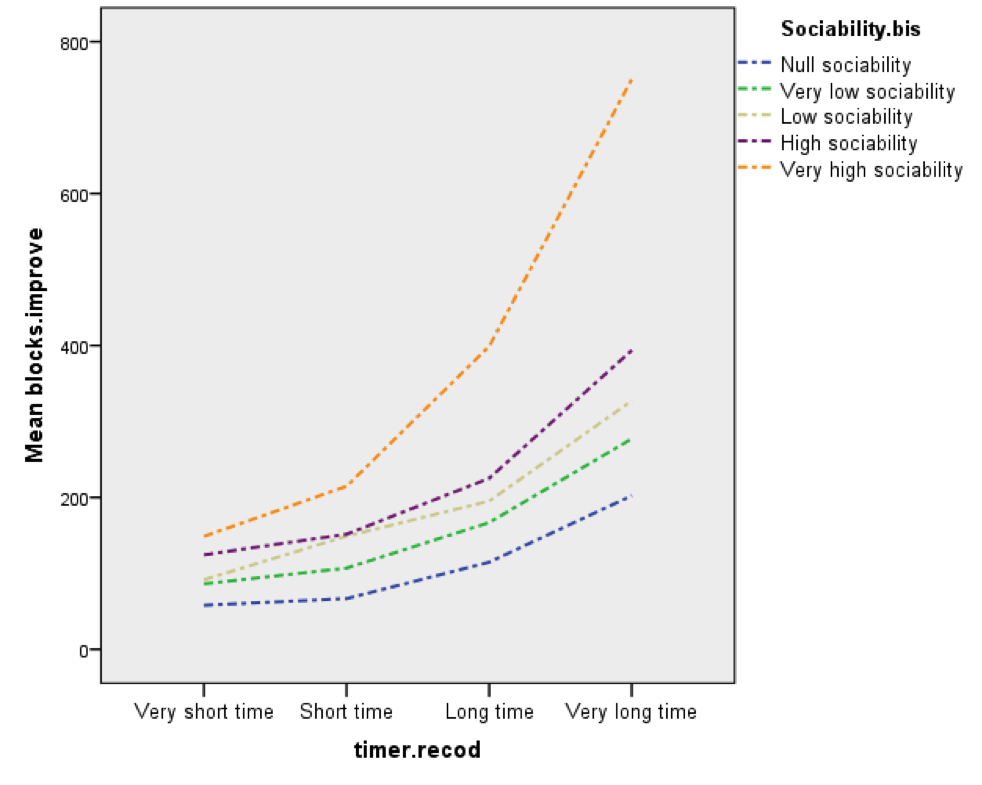
\includegraphics[width=.48\textwidth]{figs/blocks_social2.png}
\end{subfigure} 
\begin{subfigure}
  \centering
    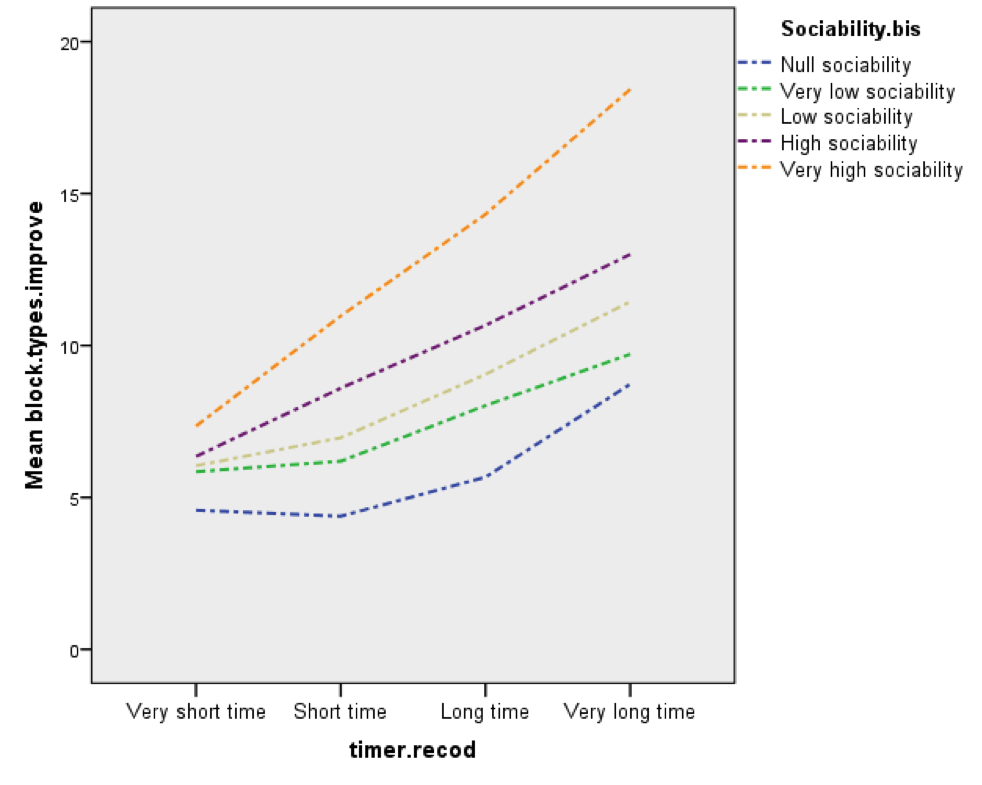
\includegraphics[width=.48\textwidth]{figs/types_social2.png}
  \caption{(l) Relationship of level of sociability with improvement in depth for each time group. (r) Relationship of level of sociability on improvement in breadth for each time group.}
  \label{fig:blocks_social2}
\end{subfigure}
\end{figure} 

\end{frame}

\usebackgroundtemplate{}


%%--------------------------------------------------------

\usebackgroundtemplate{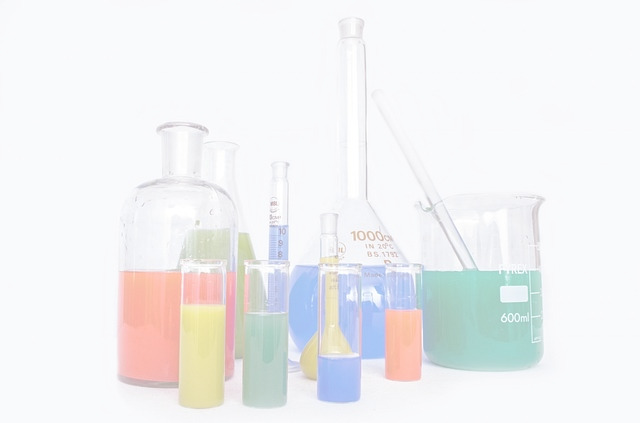
\includegraphics[height=8.8cm]{figs/research.jpg}}
%background: 

\begin{frame}
\frametitle{Research in Progress: Art with 3-year old kids}



\begin{figure}[htb!]
  \centering
  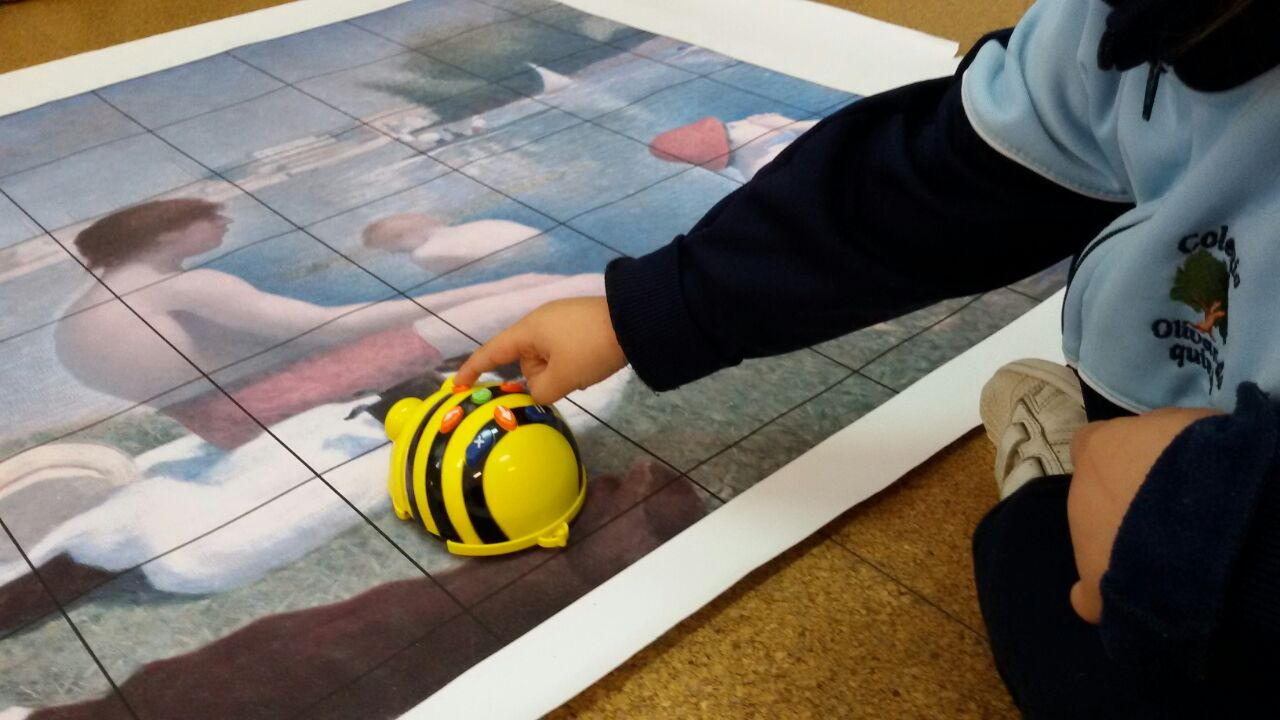
\includegraphics[width=.75\columnwidth]{figs/beebot.jpg}
  \caption{A five year old student coding a programmable robot to develop arts skills and learn about the painting \emph{Bathers at Asni�res}.}
  \label{fig:beebot}
\end{figure}


\vspace{0.2cm}
\hfill{\Tiny Background picture: Pixabay - Public domain}

\end{frame}

\usebackgroundtemplate{}



%--------------------------------------------------------

\begin{frame}
\frametitle{The quest for assessment}

  \begin{columns}[T]
    \begin{column}{0.5\textwidth}
     \begin{block}{CT-test}
\begin{figure}[t!]
\begin{center}
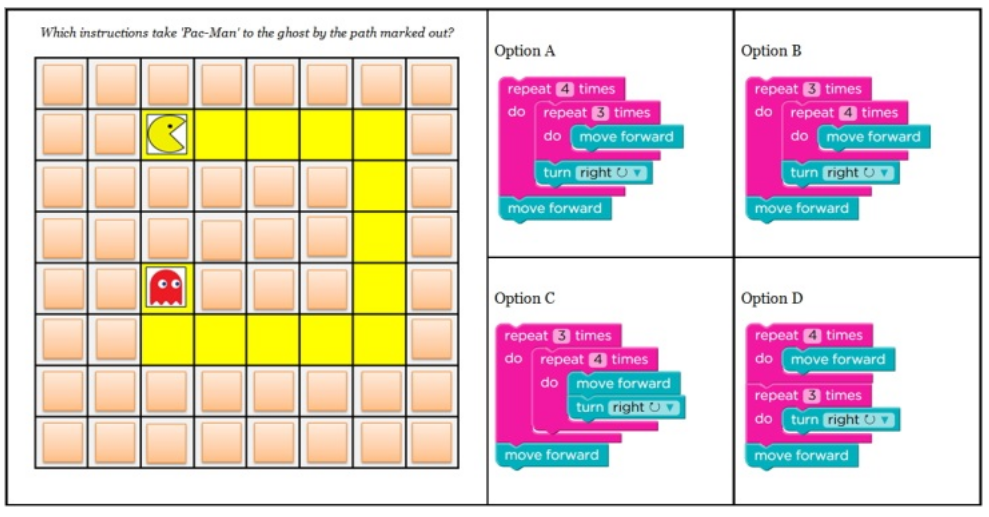
\includegraphics[width=4.8cm,height=3.6cm]{figs/comecocos.png}
\end{center}
\label{fig:cttest}
\end{figure}
\begin{center}
diagnostic-summative paper-and-pen test
\end{center}
     \end{block}
    \end{column}
    \begin{column}{0.5\textwidth}
 
     \begin{block}{Dr. Scratch}
\begin{figure}[t!]
\begin{center}
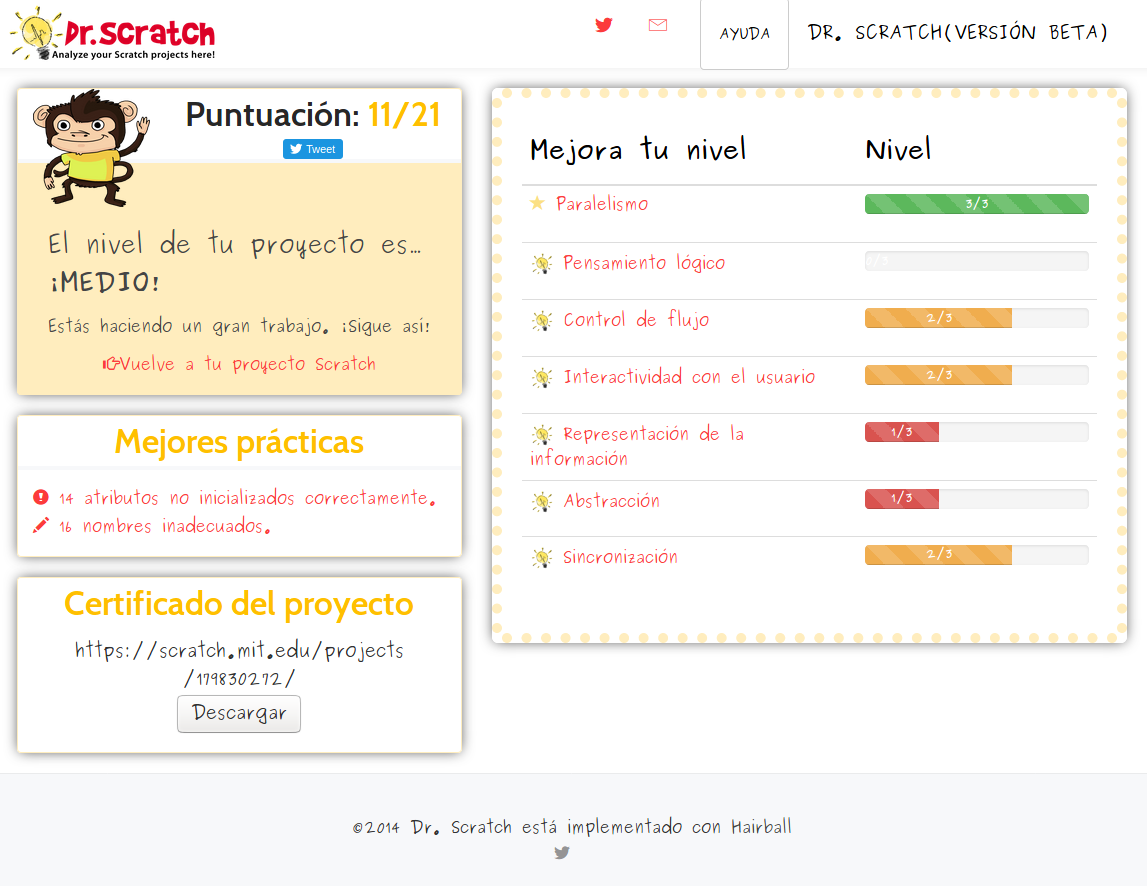
\includegraphics[width=4.8cm,height=3.6cm]{figs/drscratch2.png}
\end{center}
\label{fig:drscratch}
\end{figure}
\begin{center}
formative assessment tool
\end{center}
     \end{block}

    \end{column}
  \end{columns}
\begin{center}
Other methods exist, such as Bebras \\ (which asseses skill transference)
\end{center}


\end{frame}

\usebackgroundtemplate{}




%%--------------------------------------------------------
\usebackgroundtemplate{
\includegraphics[width=13cm]{figs/take-away.jpg}}
%% background: http://flamingcow.co.uk/wp-content/uploads/2015/02/takeaway-940x283.jpg

\begin{frame}
\frametitle{Takeaways}

  \begin{enumerate}
    \item Computational Thinking is becoming increasingly popular in recent times
    \item Focus should not be placed exclusively on programming, but on the skills
    \item We need more research on the impact of CT on other subjects, including tools that facilitate this task
    \item We need better assessment tools
  \end{enumerate}

\vspace{0.85cm}
\hfill{\Tiny Background picture: flamingcow.co.uk}
%
\end{frame}

\usebackgroundtemplate{}

%--------------------------------------------------------
\usebackgroundtemplate{
\includegraphics[width=13cm]{figs/books.jpg}}
% http://www.aspa-usa.org/wp-content/uploads/2015/06/books.jpg
\begin{frame}
\frametitle{Learn more}
\vspace{-0.65cm}
\begin{center}
\footnotesize
\begin{columns}[T]
    \begin{column}{1\textwidth}
     \begin{block}{Some references}
       \begin{itemize}
	 \item Moreno-Le\'on, J., Robles, G, \& Roman-Gonz\'alez, M. (2015). Dr. Scratch: Automatic Analysis of Scratch Projects to Assess and Foster Computational Thinking. \textit{RED. Revista de Educaci�n a Distancia, 15}(46).
	 \item Moreno-Le\'on, J., Robles, G, \& Roman-Gonz\'alez, M. (2016). Comparing computational thinking development assessment scores with software complexity metrics. In \textit{Global Engineering Education Conference (EDUCON), 2016 IEEE}. IEEE.
	 \item J. Moreno-Le�n, G. Robles, and M. Rom�n-Gonz�lez. Examining the Relationship between Socialization and Improved Software Development Skills in the Scratch Code Learning Environment. Journal of Universal Computer Science, 22(12), pp. 1533-1557, 2016.
       \end{itemize}
    \end{block}
    \end{column}
  \end{columns}
\end{center}
\end{frame}

\usebackgroundtemplate{}

\frame{
\maketitle
\begin{center}

\includegraphics[width=1.4cm]{format/intef}
\hspace{0.5cm}

\includegraphics[width=3.2cm]{format/urjc}
\hspace{0.5cm}

\includegraphics[width=1.3cm]{format/uned.jpg}
\hspace{0.5cm}

\includegraphics[width=3cm]{format/emadrid.png}
\end{center}
}


\end{document}
